\icode{E-MI-MU-L2-261108-001}
（多选）
两个劲度系数分别为\(k_1\)和\(k_2\)的轻质弹簧\(a\)、\(b\)串接在一起，\(a\)弹簧的一端固定在墙上，如图所示。开始时弹簧均处于原长状态，现用水平力作用在\(b\)弹簧的\(P\)端向右拉动弹簧，已	知\(a\)弹簧的伸长量为\(L\)，则\paren[]
	
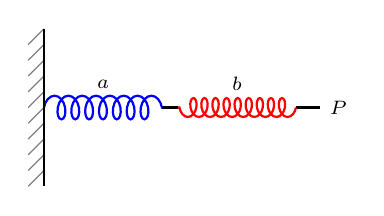
\begin{tikzpicture}[font=\scriptsize]
	\foreach \y in {1,.8,...,-.8}
		\draw[gray] (0,\y)--++(-.2,-.2);
	\draw[thick] (0,1)--(0,-1) (1.5,0)--(1.7,0) (3.2,0)--(3.5,0)node[right]{\(P\)};
	\draw[thick,decoration={aspect=.6,segment length=5,amplitude=1.5mm,coil},decorate,blue] (0,0)--(1.5,0);
	\draw[thick] (0,1)--(0,-1);
	\draw[thick,decoration={aspect=.6,segment length=4,amplitude=1.2mm,coil},decorate,red] (3.2,0)--(1.7,0);
	\node at(.75,.3){\(a\)};
	\node at(2.45,.3){\(b\)};
\end{tikzpicture}
\begin{choices}
	\item\(b\)弹簧的伸长量也为\(L\)
	\item\(b\)弹簧的伸长量也为\(\frac{k_1}{k_2}L\)
	\item\(P\)端向右移动的距离为\((1 + \frac{k_1}{k_2})L\)
	\item\(P\)端向右移动的距离为\((1 + \frac{k_2}{k_1})L\)
\end{choices}
\begin{answer}
	BC\qquad 提示：
\end{answer}